The regular training procedure for a four feature model has a significant limitation. The model does not take into account the Feed-Forward application of the prediction output.
If the trained model will have perfect input values, the output expected to be within~1 \% miss accuracy.
\begin{figure}[htbp]
    \centering
    % DST based tests
    \begin{subfigure}[b]{0.45\textwidth}
        \centering
        \includesvg[width=\linewidth]{III_Conclussion/im_compare/FUDS-val-48.svg}
        \caption{Regular training process snapshot}
        \label{subfig:regular_tr}
    \end{subfigure}
    \hfill
    \begin{subfigure}[b]{0.45\textwidth}
        \centering
        \includesvg[width=\linewidth]{III_Conclussion/im_compare/Sadykov2020-Feed.svg}
        \caption{Feed-Forward validation process snapshot}
        \label{subfig:regular_ts}
    \end{subfigure}
    \caption{Comparison between training and testing accuracies of a 4-featured based model with a default training and testing loop}
    \label{fig:regular_tr}
\end{figure}
% \begin{figure}[ht]%[htbp]
%     \centering
%     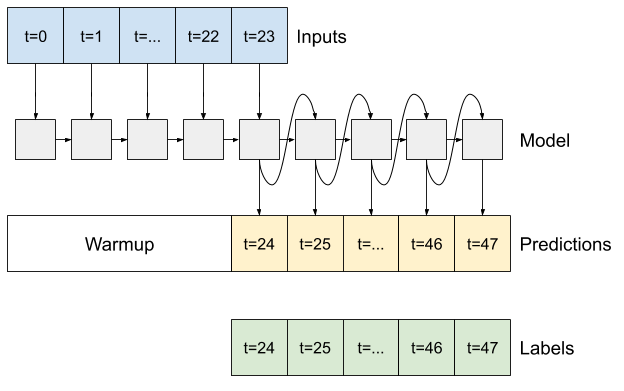
\includegraphics[width=0.7\linewidth]{II_Body/images/multistep_autoregressive.png}
%     \caption{documented way}
%     \label{fig:autoregressive}
% \end{figure}


%
%
Two subplots in figure~\ref{fig:regular_tr} demonstrate the results of the prediction of a four feature-based trained model against a single battery cycle of DST driving.
Subfigure~\ref{subfig:regular_tr} demonstrates the prediction based on the always known perfect State of Charge, opposite on subfigure~\ref{subfig:regular_ts} with only perfect initial, and every following sample gets fed-forward.
It demonstrates how the appended charge output model accumulates the error with every dependant input in a single prediction.
If that output will be used for further prediction and the model keeps preserving the dependency, the miss accuracy value rises non-linearly.
The reason for that lies in the amount of weight the model places on the State of Charge input feature.
For a better weights balance, the training procedure must be modified to consider the possibility of an inaccuracy in the input charge data.
The diagram in Figure~\ref{subfig:testing} illustrates regular training and testing procedures for a model to produce output.
\begin{figure}[htbp]
    \centering
    % DST based tests
    \begin{subfigure}[b]{0.85\textwidth}
        \centering
        % 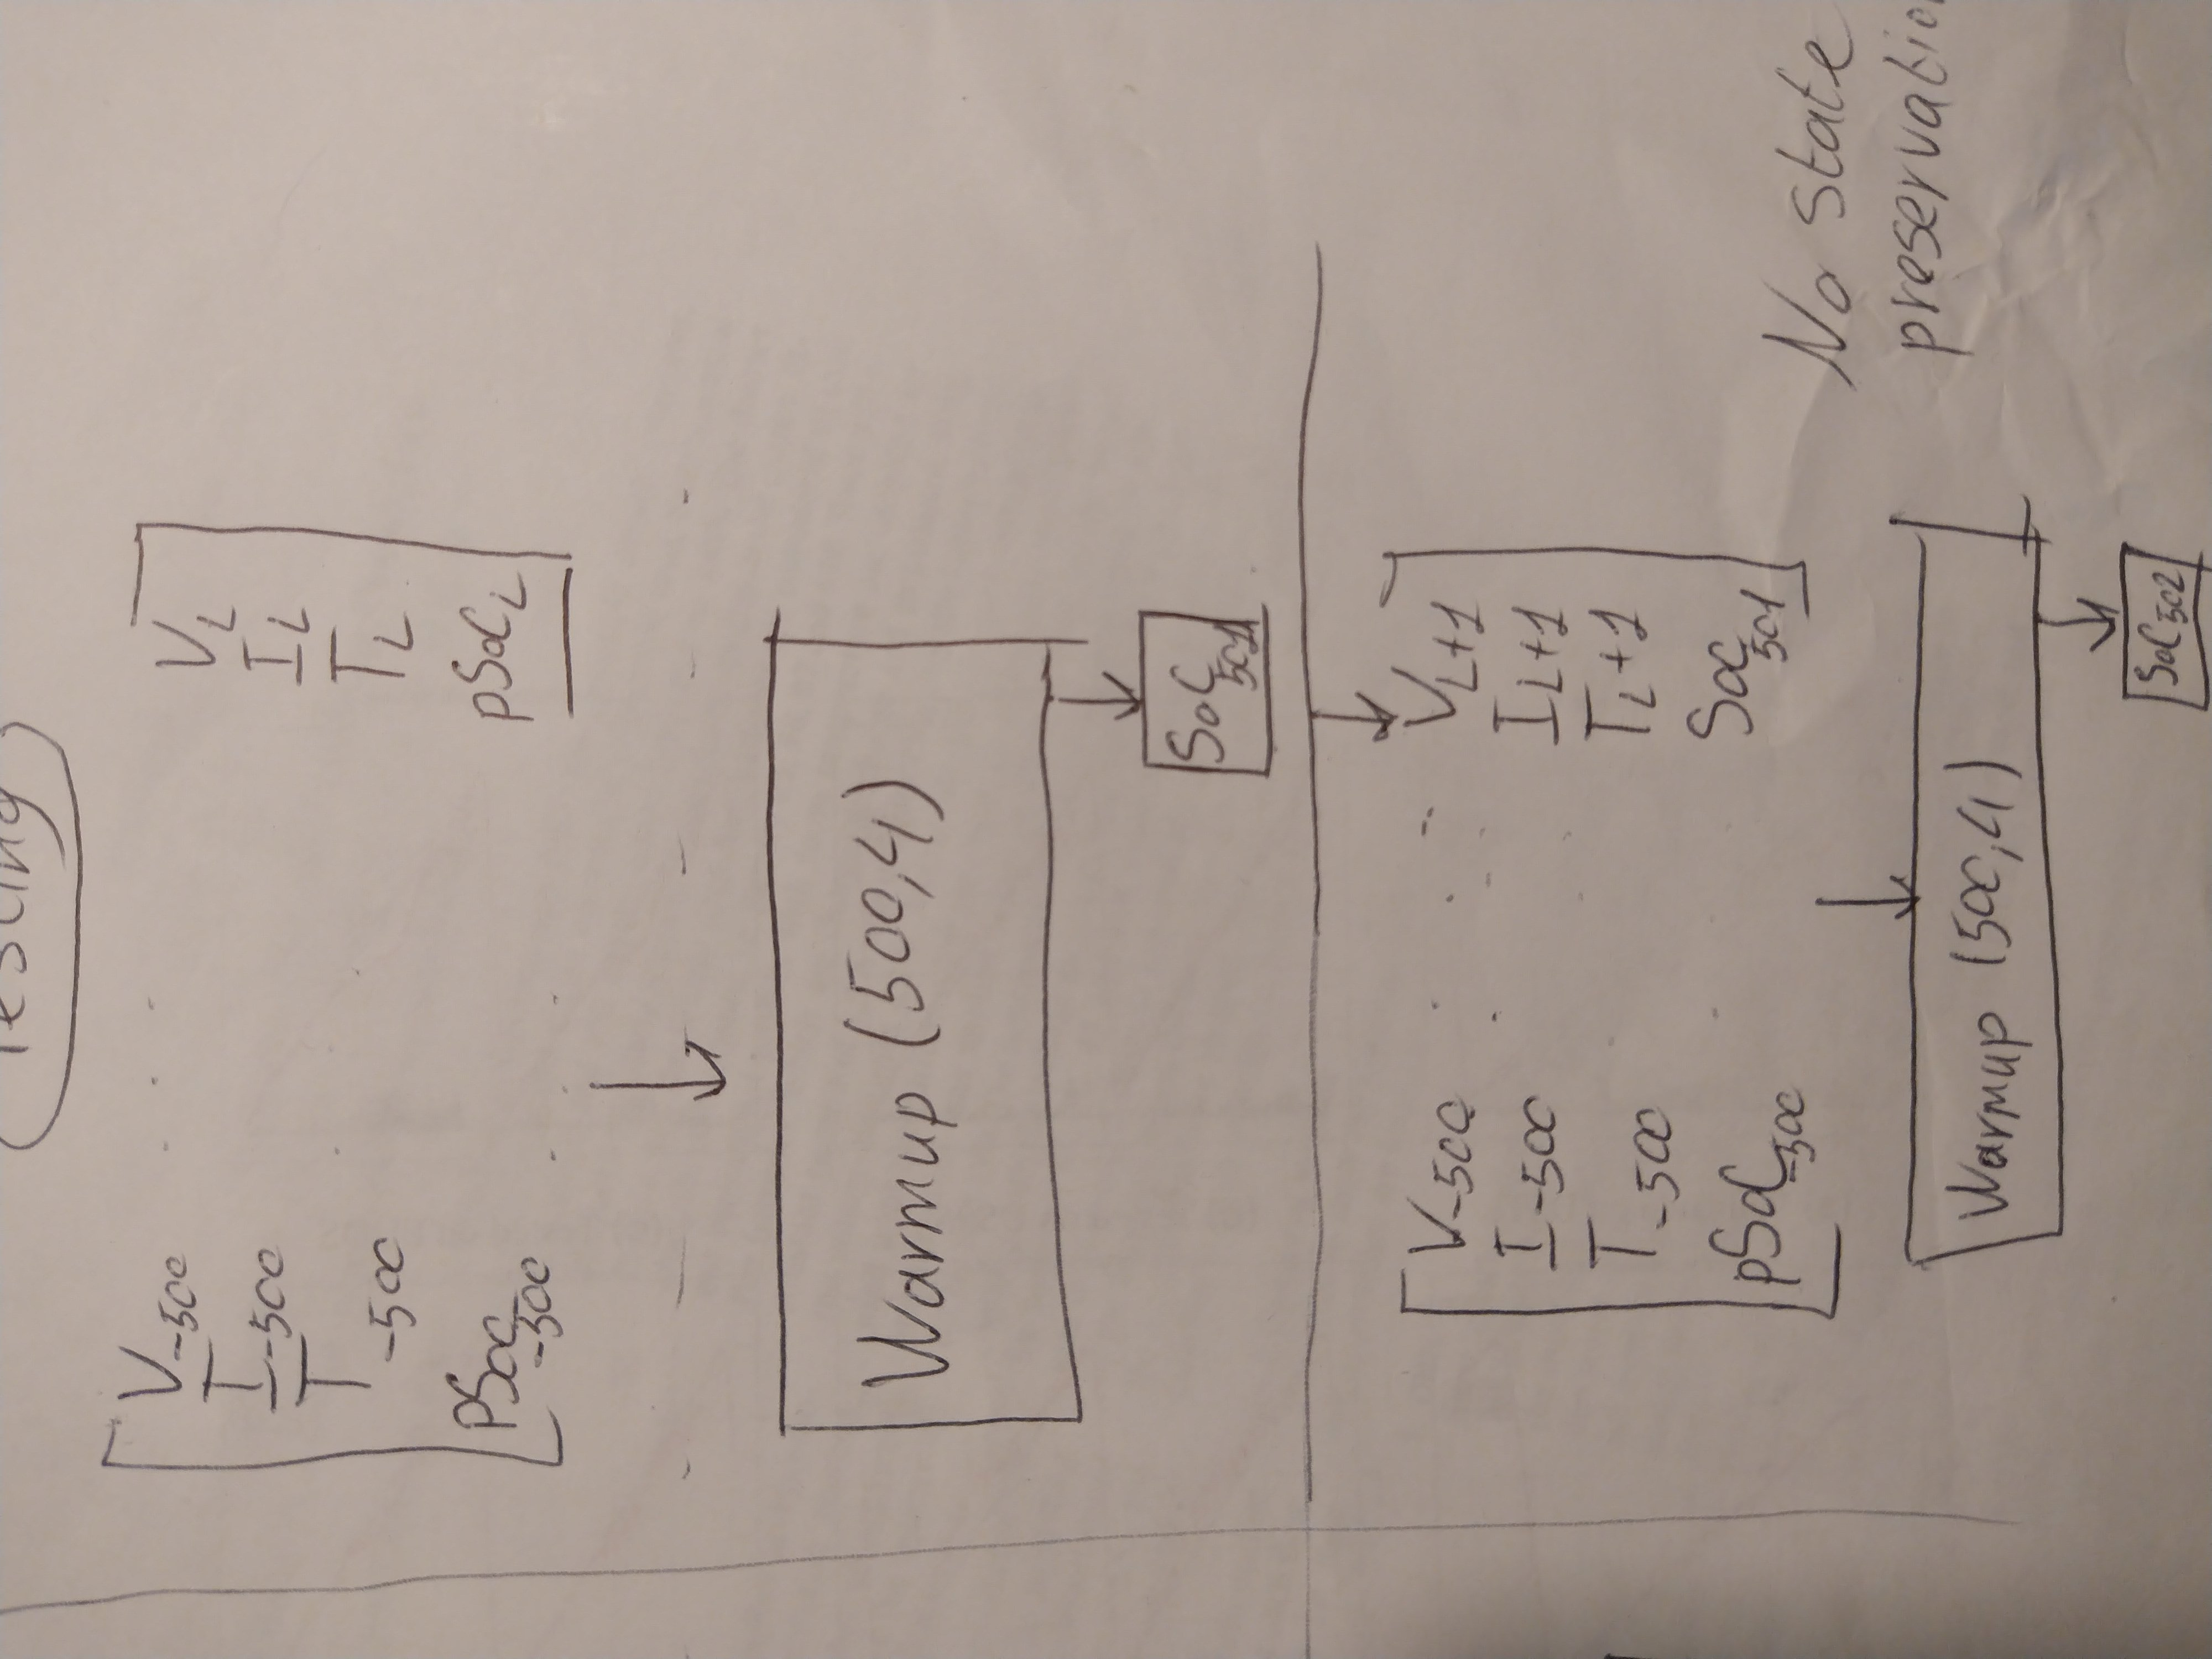
\includegraphics[width=\linewidth]{II_Body/images/IMG_20210524_133103.jpg}
        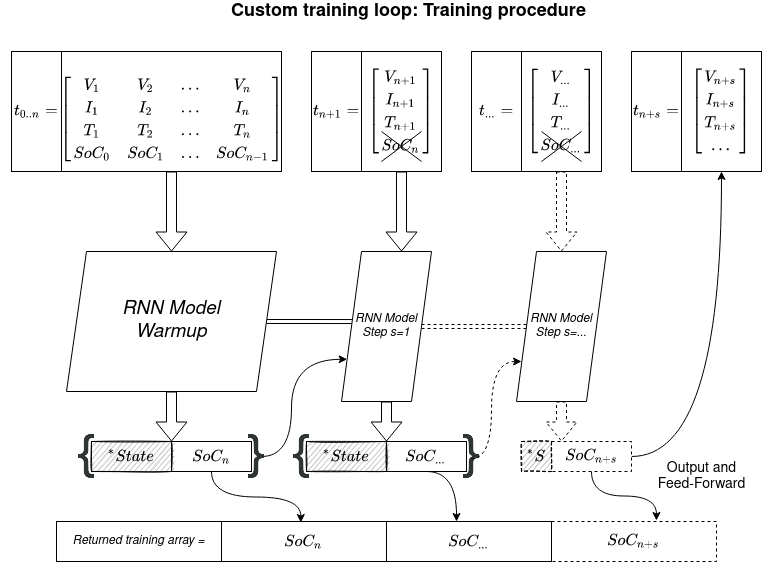
\includegraphics[width=\linewidth]{II_Body/images/Autoregression-Training.png}
        \caption{PLACEHOLDER: regular training and  procedure}
        \label{subfig:testing}
    \end{subfigure}
    \hfill
    \begin{subfigure}[b]{0.85\textwidth}
        \centering
        % 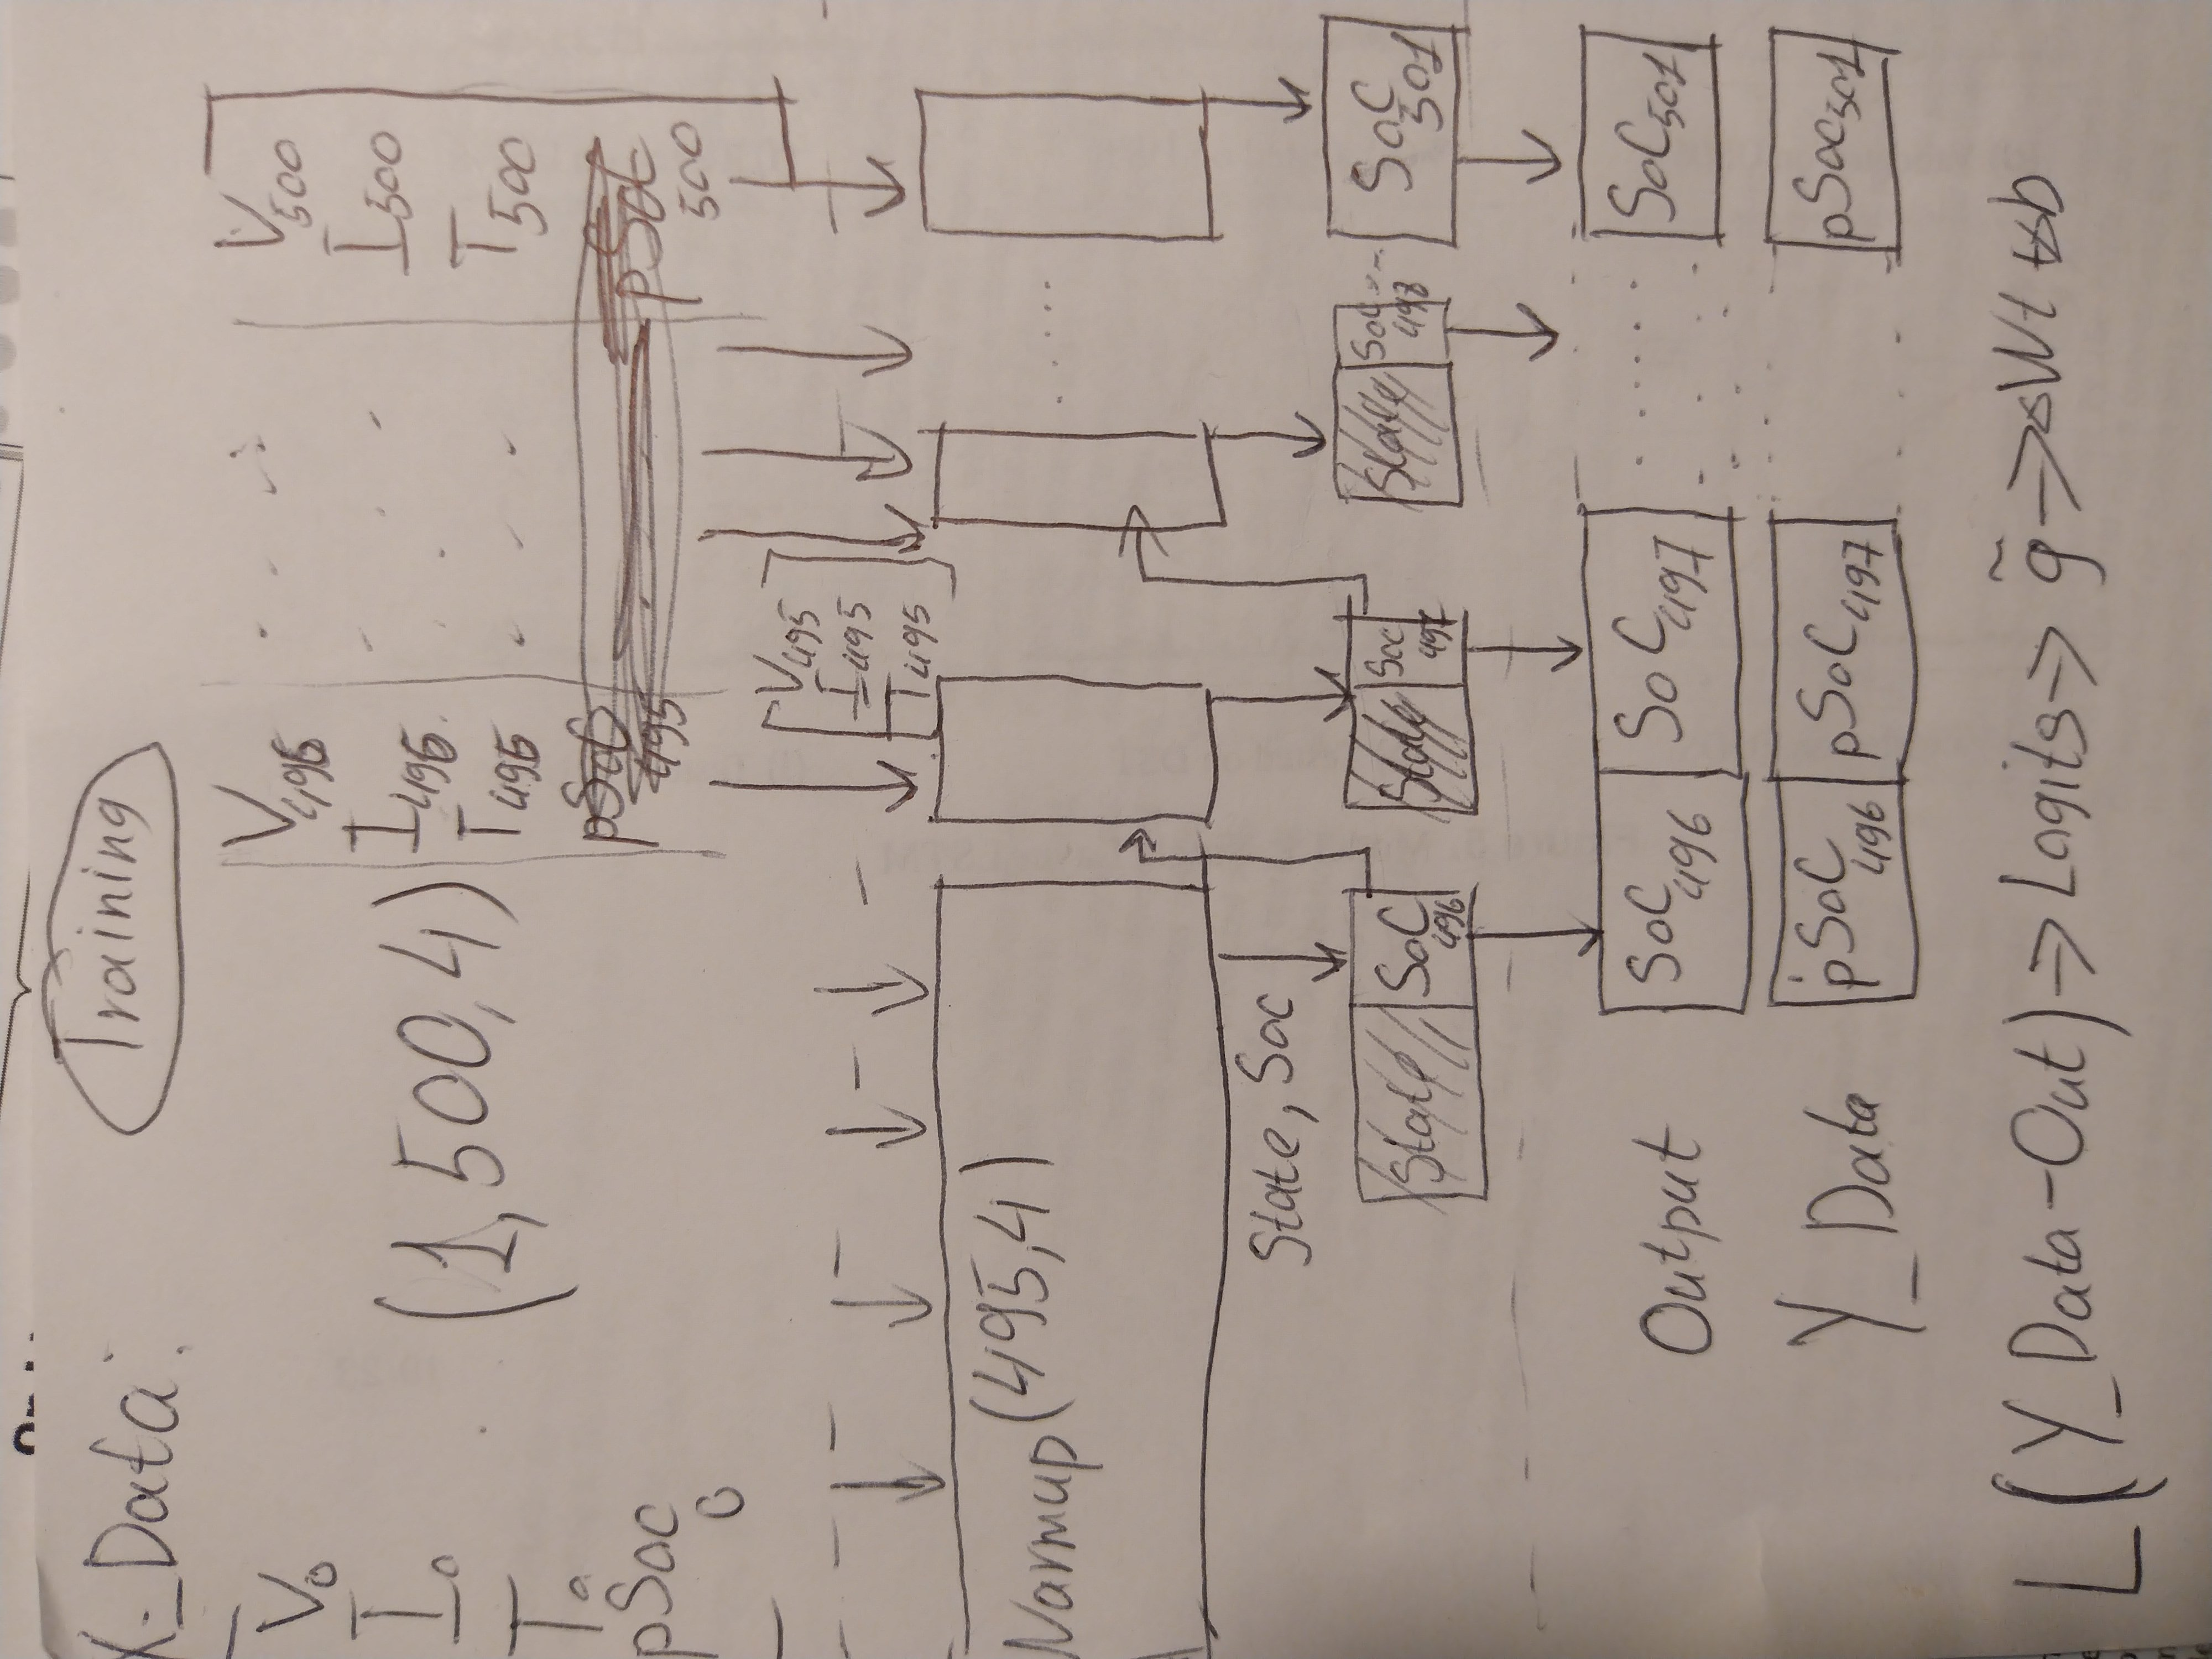
\includegraphics[width=\linewidth]{II_Body/images/IMG_20210524_133052.jpg}
        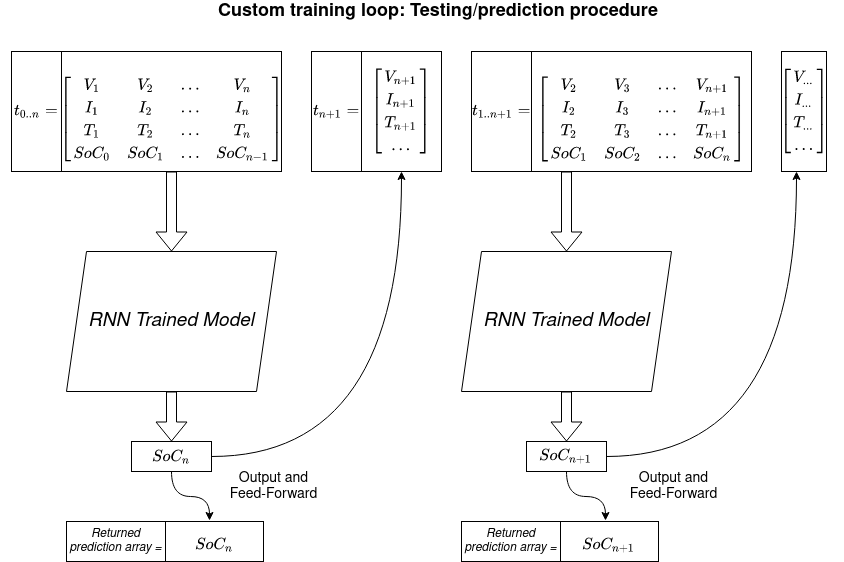
\includegraphics[width=\linewidth]{II_Body/images/Autoregression-Testing.png}
        \caption{PLACEHOLDER:testing and validation procedure}
        \label{subfig:training}
    \end{subfigure}
    \caption{Comparison between training and testing accuracy of a 4-featured based model with a default training and testing loop}
    \label{fig:training_testing}
\end{figure}

%
%
The training procedure for the regular LSTM model must be modified to consider potential inaccuracy using the autoregression technique.
\textcolor{red}{I do not feel comfortable referencing the documentation, but what choice do I have now.}
The diagram in figure~\ref{subfig:training} demonstrates the procedure for the model call using autoregression.
Unlike regular LSTM, training and testing differentiate from each other.
If the testing procedure remained unchanged, the training performs multiple calls during a single-window sample processing.
Every new call outputs the results and feeds again into the same model, with one sample from each sensor.
Each output also contained a state of the model, containing the values stored in the cell, preserving dependency between model calls.
State output used only for internal model processing.
Every output of every step has been stored as an array.
With a new approach, an optimiser will compare an array of predicted samples against the true values of the SoC.
This way meant to increase the model fit process.
The more output samples model returns during the training, the better the actual prediction against aggressive driving profiles.
Figure~\ref{fig:modefied_tr} contains a similar test as without autoregression.
Even though the accuracy with tabled samples has decreased, its feed-forward prediction accuracy has significant increase.
\begin{figure}[htbp]
    \centering
    \begin{subfigure}[b]{0.45\textwidth}
        \centering
        \includesvg[width=\linewidth]{III_Conclussion/im_compare/Sadykov2020-Normal.svg}
        \caption{Modified training process snapshot}
    \end{subfigure}
    \begin{subfigure}[b]{0.45\textwidth}
        \centering
        \includesvg[width=\linewidth]{III_Conclussion/im_time/train-iCharging.svg}
        \caption{Feed-Forward validation process snapshot on modified model}
    \end{subfigure}
    \caption{Comparison between training and testing accuracies of a 4-featured based model with a modified training and default testing loop}
    \label{fig:modefied_tr}
\end{figure}